                        %%%%%   PREAMBLE  %%%%%

\documentclass[11pt,spanish,a4paper,twoside]{article}

\usepackage[spanish,activeacute,es-noindentfirst]{babel}   % es-noindentfirst: no activa la sangr�a del primer p�rrafo tras un t�tulo
\usepackage{amssymb,amsfonts}
\usepackage{amsmath}             %  Para las f�rmula matem�ticas
\usepackage[latin1]{inputenc}    %  Permite escribir los acentos

\usepackage{fancyhdr}
\renewcommand{\headrulewidth}{0pt}  %  l�nea horiz. bajo el encabezado
\renewcommand{\footrulewidth}{0pt}  %  l�nea horiz. sobre el pie

\usepackage{makeidx}

% \usepackage{times}
% \usepackage[OT1,T1]{fontenc}

\usepackage{palatino}
% palatino: una fuente excelente, pero si sale
% mal en el .pdf descomentar las dos l�neas anterires
% y comentar �sta.

% \usepackage{charter}

\usepackage{vmargin}
\setpapersize{A4}
\setmarginsrb{2.5cm}{2cm}{2.5cm}{2cm}%
{1cm}{1cm}%
{1cm}{1cm}


\usepackage{graphicx}
\usepackage{color}       % Para el color de las fuentes
% \usepackage{lettrine}    % Letra capital
\usepackage{enumerate}   % Entorno enumerate mejorado
\usepackage{mdwlist}     % Entorno descripcion mejorado
\usepackage[amsthm,hyperref,thref]{ntheorem}
%\usepackage{paralist}


\parskip 0.15cm          % Queda mejor pero mas paginas

\input{tex/hyperref}     % Hiperreferencias

\usepackage{url}

% \usepackage{longtable}
% \usepackage{supertabular}


% \usepackage{tikz}
% \usepackage{pgf}
% \usepackage{wrapfig}

% \usepackage{placeins}   % Placeins.sty keeps floats "in their place", preventing them from floating past
                        % a "\FloatBarrier" command into another section. To use it, declare
                        % "\usepackage{placeins}" and insert "\FloatBarrier" at places that floats
                        % should not move past, perhaps at every "\section" (en "command.tex")


\usepackage[hang,footnotesize,bf]{caption}
\usepackage{subfig}
%% Entorno Descripci�n. En tres sabores:
    %% 1. El m�s general
    \newenvironment{descripcion}[2]%
    {\begin{basedescript}{\desclabelwidth{#2}}%
    \item[#1]}%
    {\end{basedescript}}%

    %% 2. Como poner en negrita (tambi�n parecido a section* pero puedo seguir en la misma l�nea)
    \newenvironment{descripcion0}[1]%
    {\begin{basedescript}{\desclabelwidth{-1ex}}%
    \item[#1]}%
    {\end{basedescript}}%

    %% 3. Con 1.25cm de tama�o
    \newenvironment{descripcion1}[1]%
    {\begin{basedescript}{\desclabelwidth{1.25cm}}%
    \item[#1]}%
    {\end{basedescript}}%

    %% Entorno para citar texto, 80% del tama�o (10% de cada lado)
      \newenvironment{citetext}{%
      \def\leftmargini{0.1\textwidth}%
      \def\rightmargini{0.1\textwidth}%
      \vspace*{-0.35cm}%
      \begin{quotation}\parskip 0.15cm\guillemotleft}%
      {\guillemotright\end{quotation}\vspace*{0.1cm}}


      %% Sin � (caso especial de citetext)
      \newenvironment{citetext_sin_right}{%
      \def\leftmargini{0.1\textwidth}%
      \def\rightmargini{0.1\textwidth}%
      \vspace*{-0.35cm}%
      \begin{quotation}\parskip 0.15cm\guillemotleft}%
      { \end{quotation}\vspace*{0.1cm}}



\newcommand{\subsubseccion}[1]{\subsubsection*{#1}\addcontentsline{toc}{subsubsection}{#1}}



% Circulos chicos: un cuarto, mitad, trescuartos y completo.
% \newcommand{\quarter}{
%                     \begin{tikzpicture}
%                     \fill[black] (0,0.11) arc (90:-90:0.1cm) ;
%                     \filldraw[white] [rotate=-90] (0,0.11) arc (90:-90:0.1cm);
%                     \draw (0,0) circle (0.1cm);
%                     \end{tikzpicture}
%                     }
% 
% \newcommand{\half}{
%                     \begin{tikzpicture}
%                     \draw (0,0) circle (0.1cm);
%                     \fill[black] (0,0.11) arc (90:-90:0.1cm) ;
%                     \end{tikzpicture}
%                    }
% 
% \newcommand{\threequarter}{
%                     \begin{tikzpicture}
%                     \fill[black] (0,0.10) arc (90:-90:0.1cm);
%                     \filldraw[black] [rotate=-90] (0,0.10) arc (90:-90:0.1cm);
%                     \draw (0,0) circle (0.1cm);
%                     \end{tikzpicture}
%                    }
% 
% 
% \newcommand{\full}{
%                     \begin{tikzpicture}
%                     \fill[black] (0,0.10) arc (180:-180:0.1cm);
%                     \end{tikzpicture}
%                      }



% Circulos grandes
\newcommand{\quarter}{
                    \begin{tikzpicture}
                    \fill[black] (0,0.16) arc (90:-90:0.9ex);
                    \filldraw[white] [rotate=-90] (0,0.16) arc (90:-90:0.9ex);
                    \draw (0,0) circle (1ex);
                    \end{tikzpicture}
                    }

\newcommand{\half}{
                    \begin{tikzpicture}
                    \fill[black] (0,0.165) arc (90:-90:0.9ex) ;
                    \draw (0,0) circle (1ex);
                    \end{tikzpicture}
                   }

\newcommand{\threequarter}{
                    \begin{tikzpicture}
                    \fill[black] (0,0.165) arc (90:-90:0.9ex) ;
                    \filldraw[black] [rotate=-90] (0,0.16) arc (90:-90:0.9ex) ;
                    \draw (0,0) circle (1ex);
                    \end{tikzpicture}
                        }


\newcommand{\full}{
                    \begin{tikzpicture}
                    \filldraw[black] [rotate=-90] (0,0.18) arc (180:-180:1ex) ;
                    \end{tikzpicture}
                     }

\makeindex

\begin{document}
    \pagestyle{headings}
                                           %%% TITULO %%%

\pagestyle{empty}   % para que no tenga n�mero
                    % (�ste es el motivo por el
                    %  cu�l no uso "\maketitle")

% \vspace*{-1.65 cm}
 \begin{center}
   \begin{Large}
%          Online Mathematical Handwriting Recognition
         \textbf{Reconocimiento de Escritura Manuscrita} \\
         \begin{footnotesize}
            \textbf{\textit{(Online Handwriting Recognition)}}
         \end{footnotesize}
   \end{Large}
 \end{center}


\vspace*{1.65 cm}
\begin{center}
  \begin{Large}
    \textit{Tesina de Grado
    \vspace*{0.1 cm} \\
    \begin{footnotesize}Septiembre 2011    \end{footnotesize}
    }
  \end{Large}
\end{center}


\vspace*{1.65 cm}
\begin{center}
  \begin{Large}
   \textsc{Pablo Speciale}
  \end{Large}
\end{center}


\vspace*{1.65 cm}
\begin{center}
    \includegraphics[scale=0.04]{imagen/logo_fceia.pdf}
    \hspace*{5cm}
    \includegraphics[scale=0.25]{imagen/logo_unr.pdf}
\end{center}


\vspace*{0.65 cm}
\begin{center}
\textit{
Lic. en Cs. de la Computaci�n \\
Facultad de Ciencias Exactas, Ingenier�a y Agrimensura \\
Universidad Nacional de Rosario}
\end{center}


\vspace*{3.5cm}
\textbf{Director}: Dr. Juan Carlos Gomez\footnote{Director del grupo \textit{Procesamiento de Se�ales Multimedia} del CIFASIS}

% \vspace{0.5cm}
\textbf{Co-director}:  Dr. Pablo Granitto\footnote{Director del grupo \textit{Aprendizaje Automatizado y Aplicaciones} del CIFASIS}


\newpage




%
%
% \topmargin 0 truecm
%
% \pagestyle{empty}
%
% \begin{center}
%
% \vskip -3.0cm
% {\LARGE \sf {\huge mcBrief}: un descriptor local de features \\ para im�genes color} \\
%
% \vspace{4.0cm}
% {\Large \sf Tesina de grado}
%
% \vspace{1.5cm}
% {\Large Autor: Daniel Moreno}
%
% \vspace{0.5cm}
% {\Large Director: Mario E. Munich}
%
% \vspace{2.4cm}
% {\large \sf Julio 2011}
%
% \vspace{2.5cm}
%
% \begin{figure}[h]
% \begin{center}
% \includegraphics[height=1.6cm]{logo_lcc.png}
% \end{center}
% \end{figure}
%
% \begin{figure}[h]
% \begin{center}
% \includegraphics[height=1.6cm,width=1.6cm]{LogoUNR.png}
% \end{center}
% \end{figure}
%
%
% {\it Lic. en Cs. de la Computaci�n \\
% Facultad de Ciencias Exactas, Ingenier�a y Agrimensura \\
% Universidad Nacional de Rosario }
%
%
% \end{center}
                            %%%%%   INDICE  %%%%%

% \setcounter{page}{1}
% \thispagestyle{empty}
\pagenumbering{roman}        % N�meros de p�ginas en Romano

\pagestyle{fancy}
\fancyhf{}                   % Borrar todos los ajustes
\fancyfoot[C]{\thepage}
% \fancyhead[RO,RE]{\scshape{\thepage}}
% \fancyhead[LO]{\scshape{�ndice General}}
% \fancyhead[LE]{\scshape{�ndice General}}
% \renewcommand{\headrulewidth}{0.1pt}

\pdfbookmark[0]{�ndice General}{tit}       %Agrega "�ndice General"' al bookmark.

\tableofcontents

\clearpage
% \cleardoublepage
                            %%%%%   ESTILO  %%%%%

\renewcommand{\headrulewidth}{0pt}  %  l�nea horiz. bajo el encabezado
\renewcommand{\footrulewidth}{0pt}  %  l�nea horiz. sobre el pie

\pagenumbering{arabic}

%
%  Simple faz
%
\pagestyle{fancy}
\fancyhf{}                   % Borrar todos los ajustes
\fancyfoot[C]{\thepage}
% \fancyhead[RO,RE]{\scshape{\thepage}}  % N�meros de p�gina en las esquinas de los encabezados
\renewcommand{\sectionmark}[1]{
    \fancyhead[RO]{\begin{footnotesize}\thesection.\ \scshape{#1}\end{footnotesize}}
    \fancyhead[RE]{\begin{footnotesize}\thesection.\ \scshape{#1}\end{footnotesize}}
    \renewcommand{\headrulewidth}{0.1pt}
}
\renewcommand{\subsectionmark}[1]{
    \fancyhead[RE]{\begin{footnotesize}\thesubsection.\ \scshape{#1}\end{footnotesize}}
}


%
%  Doble faz
%
% \pagestyle{fancy}
% \fancyhf{}                   % Borrar todos los ajustes
% \fancyfoot[C]{\thepage}
% % \fancyhead[RO,LE]{\begin{small}\thepage\end{small}}  % N�meros de p�gina en las esquinas de los encabezados
% \renewcommand{\sectionmark}[1]{
%     \fancyhead[RO]{\begin{footnotesize}\thesection.\ \scshape{#1}\end{footnotesize}}
%     \fancyhead[LE]{\begin{footnotesize}\thesection.\ \scshape{#1}\end{footnotesize}}
%     \renewcommand{\headrulewidth}{0.1pt}
% }
% \renewcommand{\subsectionmark}[1]{
%     \fancyhead[RE]{\begin{footnotesize}\thesubsection.\ \scshape{#1}                   \end{footnotesize}}
% }


%% Para los perzonalizar itemize
\renewcommand{\labelitemi}{$\bullet$}
\renewcommand{\labelitemii}{$\ast$}


% % A more convenient way to stop floats at section boundaries is to change
% % the definition of "\section" to include "\FloatBarrier", at the beginning
% \let\oldsection\section
% \renewcommand{\section}{\FloatBarrier\oldsection}


% % Util para ser impreso. Hace que las secciones comiencen desde una p�gina impar
% % similar a \cleardoublepage
% \let\oldsection\section
% \renewcommand{\section}{\cleartoevenpage\oldsection}


    \pagestyle{fancy}

% \titlespacing*{\section}{0pt}{1.5ex}{1.5ex}

%     \section{Introducci�n}

\subsection{Motivaci�n}
% \noindent
Actualmente es posible escribir en dispositivos electr�nicos, sobre todo con la llegada de las Tablet PC, pizarras el�ctricas, celulares touch-screen y las pantallas t�ctiles. Tambi�n cabe destacar algunos e-Readers que permiten la escritura, convirti�ndose en \textit{papel electr�nico}. La escritura se realiza generalmente con un \textit{stylus} (l�piz), abriendo la puerta a nuevas interacciones m�s all� del teclado y mouse. En la figura \ref{tabletas}, puede apreciarse una variedad de dispositivos que permiten la escritura con l�piz.
\begin{figure}[!htbp]
 \centering
 \includegraphics[scale=0.65]{imagen/tabletas.pdf}
 \caption{Tabletas}
 \label{tabletas}
\end{figure}

A pesar de que exista una variedad importante de tales dispositivos, no hay todav�a una aplicaci�n sobresaliente de reconocimiento para ellos. El usuario ve al \textit{stylus} como un mouse sofisticado, sin que se logre una mejora significativa en la productividad al no explotar la potencialidad del mismo. Un buen sistema de reconocimiento de escritura (\textit{handwriting recognition}\footnote{Muchos t�rminos utilizados aqu� se dejan intencionalmente en ingl�s, facilitando la b�squeda de contenido para tales t�rminos.}) podr�a permitir al usuario una mejor experiencia con respecto al papel y l�piz tradicional, permiti�ndole obtener resultados inmediatos a partir de su escritura, como ser resultados matem�ticos.


\vspace*{-0.15cm}
\subsection{Organizaci�n del trabajo}
\vspace*{-0.1cm}
En la secci�n \ref{sec:Conceptos_Generales}, se introducen los conceptos generales de reconocimiento de escritura; en la secci�n \ref{fundamentos}, se introducen los fundamentos te�ricos en los que se basa el trabajo; en la secci�n \ref{feature_extraction}, se explica la extracci�n de caracter�sticas; en la secci�n \ref{clasificacion}, se comentan los m�todos de clasificaci�n utilizados; en la secci�n \ref{sec:resultados}, se comparan todos los m�todos; en la secci�n \ref{sec:aplicaciones}; se provee una visi�n futura de las posibles aplicaciones de los m�todos explicados; y por �ltimo, en la secci�n \ref{sec:conclusion}, se presentan algunas conclusiones.

    \section{Conceptos Generales}

En esta secci�n se describir�n las partes esenciales del campo permitiendo as� aclarar en d�nde se centrar� este trabajo. Tambi�n se comentar� brevemente las etapas que intervienen en el proceso de reconocimiento de escritura (\textit{handwriting recognition}\footnote{Muchos t�rminos utilizados aqu� se dejan intencionalmente en ingl�s, facilitando la b�squeda de contenido de tales t�rminos.}).
% que tiene un sistema de reconocimiento de escritura.


% En esta secci�n describir las partes esenciales del campo y reducirlo para 
% ubicar al lector para que pueda entender en que parte del campo se trabaj�.

% se intenta reducir el campo de handwriting recognition de manera que se pueda apreciar en qu� parte del campo se est� trabajando. Tambi�n se describen las etapas en las cu�les se debe profundizar.

% se centralizar�
% para centrarlo en un subdominio 

% focalizar�
% reducir�


\subsection{Motivaci�n}
% \noindent
Actualmente es posible escribir en dispositivos electr�nicos, sobre todo con la llegada de las Tablet PC, pizarras el�ctricas, celulares touch-screen y las pantallas t�ctiles. Tambi�n cabe destacar algunos e-Readers que permiten la escritura, convirti�ndose en \textit{papel electr�nico}. La escritura se realiza generalmente con un \textit{stylus} (l�piz), abriendo la puerta a nuevas interacciones m�s all� del teclado y mouse. En la figura \ref{tabletas}, puede apreciarse una variedad de dispositivos que permiten la escritura con l�piz.
\begin{figure}[!htbp]
 \centering
 \includegraphics[scale=0.70]{imagen/tabletas.pdf}
 \caption{Tabletas}
 \label{tabletas}
\end{figure}

A pesar de que exista una variedad importante de tales dispositivos, todav�a no hay una aplicaci�n sobresaliente de reconocimiento para ellos. El usuario ve al \textit{stylus} como un mouse sofisticado, sin que se logre una mejora significativa en la productividad al no explotar la potencialidad del mismo. Un buen sistema de \textit{handwriting recognition} podr�a permitir al usuario una mejor experiencia con respecto al papel y l�piz tradicional, permiti�ndole obtener resultados inmediatos a partir de su escritura, como ser resultados matem�ticos.


\vspace*{-1ex}
\subsection{Reconocimiento Online vs Offline}
\label{Fundamentos}

% \subsubsection{On-line vs Off-line}
% \noindent
A diferencia del enfoque \textit{Offline} de handwriting recognition, el cual pretende reconocer caracteres a partir de una imagen, el enfoque \textit{Online} intenta el reconocimiento a partir de secuencias de puntos, aqu� llamados trazos (\textit{strokes}). Ambos enfoques est�n esquem�ticamente representados en la figura \ref{fig:off|on-line}.
\begin{figure}[!htbp]
 \centering
 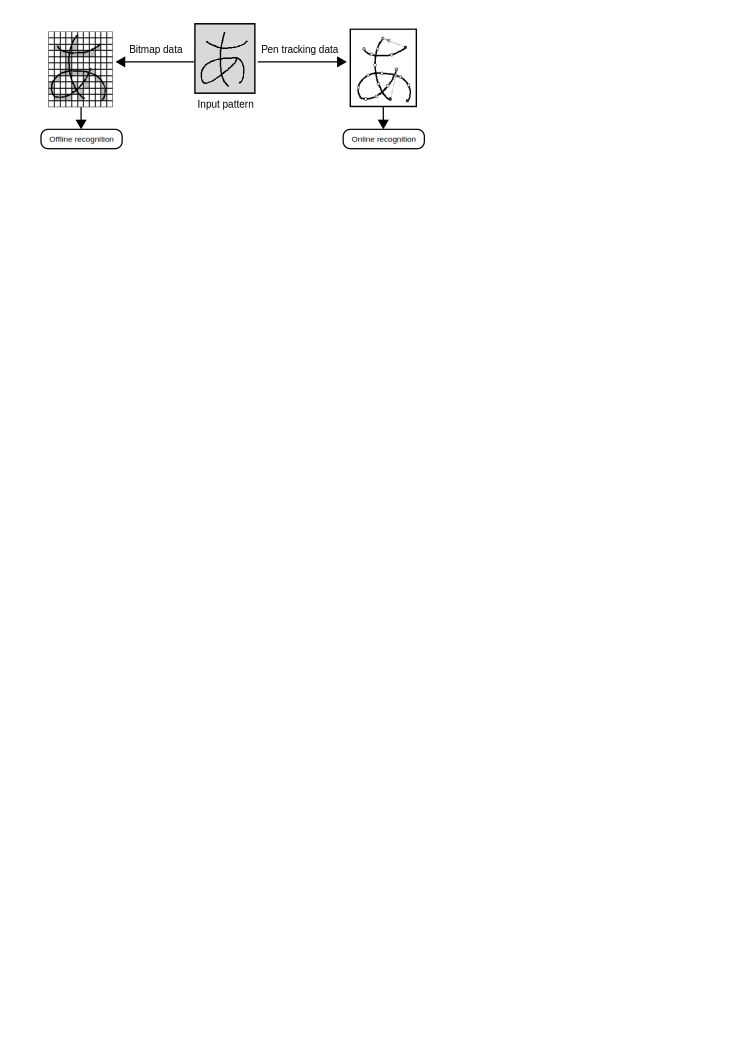
\includegraphics[scale=0.85]{imagen/off|on-line.pdf}
 \caption{Offline vs Online.}
 \label{fig:off|on-line}
\end{figure}

Como puede verse, se posee el orden en que cada uno de los puntos fue escrito. As�, es posible diferenciar distintos estilos de escrituras, a pesar de que el resultado final puede que sea el mismo. La utilizaci�n de un stylus en un dispositivo electr�nico permite usar el enfoque Online.


\subsection{Segmentaci�n}
\label{segmentation}
% \noindent
Se asume que la escritura est� en imprenta y los s�mbolos est�n bien distanciados entre s�. Seg�n la figura \ref{fig:segmentation}, nuestra hip�tesis es la utilizaci�n del nivel 2 de segmentaci�n en la construcci�n de la base de datos. Las dem�s formas de escritura requieren de un trabajo adicional de segmentaci�n que no entra en el alcance de este trabajo.
\begin{figure}[!htbp]
 \centering
 \includegraphics[scale=0.75]{imagen/segmentation.pdf}
 \caption{Niveles de dificultad en segmentaci�n \cite{Connell00onlinehandwriting}.}
 \label{fig:segmentation}
\end{figure}



\subsection{Etapas de reconocimiento de escritura}
\noindent
En el an�lisis \textit{handwriting recognition} pueden reconocerse las siguientes posibles etapas:
% , como en parte se destaca en \cite{CommunicatingMathematics}:

\begin{enumerate}[1.]

 \item \textbf{Colecci�n de trazos:}
Un s�mbolo\footnote{Se usa el t�rmino \textit{s�mbolo} en vez de \textit{caracter} pues puede ser un d�gito, una letra o un s�mbolo matem�tico.} puede ser escrito con un s�lo trazo (\textit{Single-Stroke}) o con muchos (\textit{Multi-Stroke}), ver figura \ref{fig:single|multi-stroke}. El problema de determinar qu� trazos pertenecen a qu� caracteres es llamado \textit{Stroke grouping}. Observar que esta etapa depende de la segmentaci�n asumida, ver secci�n~\ref{segmentation}.
\begin{figure}[!htbp]
 \centering
 \includegraphics{imagen/single|multi-stroke.pdf}
 \caption{Los dos primeros trazos son Single-Stroke, y el �ltimo es Multi-Stroke.}
 \label{fig:single|multi-stroke}
\end{figure}


 \item \textbf{Preproceso:}
    En el preprocesado pueden aplicarse diferentes tipos de filtros. El \textit{suavizado} elimina el ruido frecuentemente presente al principio y final de cada trazo. La normalizaci�n por \textit{resampling} ayuda a unificar distancias entre los puntos, y la normalizaci�n por \textit{resizing} asegura que el tama�o del caracter escrito no afecte al resultado del reconocimiento. En la figura \ref{fig:preprocesing} puede observarse una posible secuencia de aplicaci�n de filtros.

    \begin{figure}[!htbp]
    \centering
    \includegraphics{imagen/preprocesing.pdf}
    \caption{\texttt{(a)} Suavizado y Resizing, \texttt{(b)} Resampling }
    \label{fig:preprocesing}
    \end{figure}


 \item \textbf{Extracci�n de caracter�sticas (\textit{Feature extraction}):}
    En este paso se extraen caracter�sticas (\textit{features}) de los trazos. Hay varios tipos de features que se han usado tradicionalmente: los relativos a la apariencia que incluye, por ejemplo, proporci�n entre altura y ancho; los relativos a propiedades geom�tricas, como ser la cantidad de loops e intersecciones, centro de gravedad, puntos dominantes; los relativos al estilo de escritura, como la direcci�n y cantidad de strokes. Se posterga para la secci�n~\ref{feature_extraction} la explicaci�n de los features utilizados en este trabajo.


 \item \textbf{Entrenamiento (\textit{Training}):}
    Se requiere tener una base de datos de modelos con el cu�l contrastar el s�mbolo actual de entrada. Se realiza por una �nica vez en los algoritmos que permiten entrenamiento.
%     Y si se quiere pensarlo as�, realmente esta etapa no es parte del reconocimiento de la entrada actual en s�.


 \item \textbf{Reconocimiento o Estimaci�n (\textit{Matching}): }
    Aqu� se intenta estimar, para la entrada actual, cu�l modelo es el m�s ``similar'', sobre la base de datos disponible que sirvi� de entrenamiento. Es decir, se clasifica a la nueva entrada determinando a qu� clase pertenece. Pueden considerarse m�ltiples estimaciones, por ejemplo, dar las mejores tres estimaciones; pero en este trabajo solo se considera la primera (\textit{first match}).

\end{enumerate}


\subsection{Dependiente o independiente del usuario}
    Un sistema de \textit{handwriting recognition} puede ser dividido en: dependiente del usuario (\textit{writer-dependient}) o independiente del usuario (\textit{writer-independient}). Un sistema \textit{writer-independient} es entrenado para reconocer una gran variedad de estilos de escritura, mientras que un sistema \textit{writer-dependient} es entrenado para reconocer a un �nico individuo. Un sistema \textit{writer-dependient} trabaja con datos con poca variabilidad, y entonces puede alcanzar mejores resultado, el �nico problema es que exige al usuario tomarse el tiempo para entrenar el sistema.

    En este trabajo se puede utilizar ambos enfoques, dependiendo solo de la base de datos utilizada.


    \section{Fundamentos}
\label{fundamentos}

En esta secci�n se introducir� algunos conceptos b�sicos que utilizaremos a lo largo del trabajo.


\subsection{Preliminares}

Sea una familia de funciones $\{B_i\}$ en el espacio de funciones continuas en $[a,b]$, se definen

\begin{descripcion1}{Producto interno:}
\begin{align}
\label{def:inner_product}
 \langle B_i, B_j \rangle & \doteq \int_{a}^{b}{B}_{i}(t) \,{B}_{j}(t) \, w(t) dt
\end{align}
\end{descripcion1}

\begin{descripcion1}{Norma:}
\begin{align}
\label{def:norma}
 \| B_i \| & \doteq \sqrt{ \langle B_i, B_i \rangle }
\end{align}
\end{descripcion1}

\begin{descripcion1}{Kronecker delta:}
\begin{align}
\delta_{ij} =
        \left\{
            \begin{array}{ll}
                1 & \mbox{si } i = j \\
                0 & \mbox{si } i \neq j
            \end{array}
        \right.
\end{align}
\end{descripcion1}

\subsubsection*{Ortogonalidad:}
Se dicen que $B_i$ y $B_j$ son ortogonales si se cumple que $\langle B_i, B_j \rangle = 0$

\subsubsection*{Ortogonalizaci�n de Gram-Schmidt:}
Sea $\{v_1, \dots, v_n\}$ una base de un espacio $U$ con producto interno, se define recursivamente
\begin{align}
\label{eq:Gram-Schmidt}
u_i & = \left( v_i - \sum_{i=0}^{i-1}{\langle v_i, u_j\rangle u_j} \right)
\end{align}
Entonces, $\{u_1, \dots, u_n\}$ una base ortogonal y $\left\{\frac{u_1}{\|u_1\|}, \dots, \frac{u_n}{\|u_n\|}\right\}$ es base ortonormal de $U$.


\subsection{Polinomios ortogonales}
Polinomios ortogonales son clases de polinomios $\{B_{i}(t)\}$ definidos sobre el dominio $[a,b]$ que obedecen la relaci�n de ortogonalidad
\begin{align}
\label{eq:ortogonalidad}
\int_{a}^{b}{B}_{i}(t) \,{B}_{j}(t) \, w(t) dt & = 0 \quad\quad \text{cuando $i \neq$} j
\end{align}
donde $w(t)$ es una funci�n peso. Si adem�s cumplen con
\begin{align}
\label{eq:ortonormalidad}
 \int_{a}^{b}{B}_{i}(t) \,{B}_{j}(t) \, w(t) dt & = \delta_{ij}
\end{align}
los polinomios son \textit{\textbf{ortonormales}}. Es decir, est�n normalizados: $ \| B_i \| = 1$


% La tabla \ref{table:polinomios} muestra algunos ejemplos de los polinomios ortogonales: \\
% \begin{table}[!htbp]
% \centering
%     \begin{tabular}{ | l |c |c | c |}
%     \hline
%     \hline
%     \textbf{Polinomio} & dominio & $w(t)$ & $c_{n}$ \\
%     \hline
%     Chebyshev  & $[-1,1]$ & $(1-t^2)$ & $  $ \\[1ex]
%     Legendre   & $[-1,1]$ & $1$       & $ \frac{2}{2\,n+1} $ \\[1ex]
%     Jacobi     & $(-1,1)$ & $(1-t)^{\alpha}\,(1+t)^{\beta}$ & $ $ \\[1ex]
%     \hline
%     \hline
%     \end{tabular}
% \label{table:polinomios}
% \caption{Ejemplos de polinomios ortogonales}
% \end{table}




\subsubsection{Polinomios de Legendre}
\label{legendre}
% Son polinomios ortogonales definidos en $[-1,1]$. Se sabe que el grado de $L_i$ es exactamente $i$,  entonces pueden escribirse como

Si tomamos como funci�n peso $w(t)=1$ en la definici�n \refEQ{def:inner_product} de producto interno, es decir,
\begin{align*}
 \langle L_i, L_j \rangle & = \int_{-1}^{1}{L}_{i}(t) \,{L}_{j}(t)\,w(t)\,dt = \int_{-1}^{1}{L}_{i}(t) \,{L}_{j}(t)\,dt
\end{align*}
se pueden generar los polinomios de Legendre $\{L_i\}$ con el proceso de ortogonalizaci�n de Gram-Schmidt \refEQ{eq:Gram-Schmidt} en el intervalo $[-1,1]$. Normalizando de tal manera que $L_n(1)=1$ da los polinomios de Legendre esperados. Algunos de ellos:
\begin{align*}
L_0(t) &= 1 \\[1ex]
L_1(t) &= t \\
L_2(t) &= \frac{3\,{t}^{2}-1}{2} \\
L_3(t) &= \frac{5\,{t}^{3}-3\,t}{2} \\
L_4(t) &= \frac{35\,{t}^{4}-30\,{t}^{2}+3}{8} \\
 &~ ~\vdots
\end{align*}

% \subsubsection*{Shifted Legendre Polynomials}
Para nuestro prop�sito es conveniente utilizar los polinomios an�logos definido en $[0,1]$, los cuales son llamados \textit{\textbf{shifted} Legendre polynomials},
\begin{align}
\label{eq:legendre}
L_i(t) &= \sum_{j=0}^{i}{ C_{ij}\,t^j }
\end{align}
% donde los coeficientes $C_{ij}$ pueden calcularse con una f�rmula cerrada, ver \cite{abramowitz70a}
el grado de $L_i$ es exactamente $i$.  Se conoce una f�rmula cerrada para el c�lculos de los coeficientes $C_{ij}$ ortonormales. A continuaci�n dicha f�rmula, que puede encontrarse en \cite{abramowitz70a},
\begin{align}
\label{eq:legendre_coefficients}
C_{ij} &= (2\,i+1)^{\frac{1}{2}}\begin{pmatrix}i\cr j\end{pmatrix} {\left( -1\right) }^{j} \begin{pmatrix}j+i\cr j\end{pmatrix}
\end{align}

% \noindent
Pueden verse los primeros diez polinomios de Legendre gr�ficamente en la figura~\ref{fig:legendre}.
\begin{figure}[!htbp]
\vspace*{-0.6cm}
\centering
\includegraphics[scale=0.275]{imagen/legendre.pdf}
\vspace*{-0.6cm}
\caption{Primeros diez polinomios de Legendre (shifted) en $[0,1]$}
\label{fig:legendre}
\end{figure}


% \begin{align}
% \begin{split}
% \label{eq:legendre}
% L_i(t) &= \sum_{j=0}^{i}{ C_{ij}\,t^j }\\
% \text{donde} \quad C_{ij} &= (2\,i+1)^{\frac{1}{2}}\begin{pmatrix}i\cr j\end{pmatrix} {\left( -1\right) }^{j} \begin{pmatrix}j+i\cr j\end{pmatrix}
% \end{split}
% \end{align}


\subsubsection{Polinomios de Chebyshev}

(falta)

\subsubsection{Polinomios de Legendre-Sobolev}

(falta)

\subsection{Series de funciones ortogonales}
\label{Series_de_funciones_ortogonales}
\noindent
Si $\{B_i\}$ es una base de polinomios ortonormales respecto al producto interno \refEQ{def:inner_product},
%$L^2[a,b]$,
una funci�n continua~$f$ en el dominio $[a,b]$ puede ser escrita como
\[ f(t) = \sum_{i=0}^{\infty}{\alpha}_{i}\,{B}_{i}(t) \]
Al aplicar el producto interno con $B_i$ en ambos lados de la ecuaci�n anterior se obtiene:
\begin{align*}
\langle f, B_i \rangle & =   \left\langle \sum_{i=0}^{\infty}{\alpha}_{i}\,{B}_{i}(t), B_{i}(t) \right\rangle
                         =   \sum_{i=0}^{\infty} {\alpha}_{i} \langle {B}_{i}, B_i \rangle
                         =   \sum_{i=0}^{\infty} {\alpha}_{i} \delta_{ij}
                         =   {\alpha}_{i}
\end{align*}
Reescribiendo,
\begin{align}
\label{eq:alpha_inner_prod}
{\alpha}_{i} & = \langle f, B_i \rangle
\end{align}
\noindent
Entonces, se puede obtener una aproximaci�n a $f(t)$ al truncar la serie en un cierto orden $d$,
\begin{align}
% \begin{split}
\label{eq:aprox}
f(t) & \approx \sum_{i=0}^{d}{\alpha}_{i}\,{B}_{i}(t)
%      & =  \sum_{i=0}^{d}\langle f, B_i \rangle\,{B}_{i}(t)
\end{align}

    \section{Feature extraction}
\label{feature_extraction}

Las t�cnicas usuales para \textit{handwriting recognition} tratan de encontrar \textit{features} particulares sobre un conjunto de s�mbolos, citemos por ejemplo los d�gitos. Pero al cambiar dicho conjunto, estos features dejan de ser efectivos, no discriminan correctamente. Se vuelve impr�ctico desarrollar heur�sticas para reconocer features espec�ficos para cada s�mbolo.
% Sobre todo si se tiene en cuenta que s�mbolos matem�ticos pueden ser inventados o agregados en la marcha.
Por lo que es deseable buscar una representaci�n que permita ser aplicada sin importar qu� tipo de s�mbolo se trate; ya sea un d�gito, una letra o un s�mbolo matem�tico.

Unos de los mayores problemas con los m�todos de reconocimientos tradicionales es que los trazos son tratados como secuencias de puntos (en \textit{discreto}), en vez de verlos como lo que realmente son, curvas (en \textit{continuo}).
% son pensados como una secuencia de puntos. El problema con �sto es que no se lo est�n tratando como lo que realmente son, curvas.

\subsection{Trazos discretos como curvas continuas}
\label{Trazos_como_curvas_continuas}

En vez de describir a los trazos como una secuencia de puntos, �stos pueden ser representados por aproximaciones de curvas, figura~\ref{fig:trazos_vs_curvas}. Se mostrar� que se necesitan menos de vein\-tes~($20$) coeficientes de una serie para representar un trazo.
% \vspace*{-0.1cm}
    \begin{figure}[!htbp]
    \centering
    \includegraphics[scale=0.4]{imagen/trazos_como_curva.pdf}
%     \includegraphics[scale=0.23]{imagen/x_e_y_en_t.pdf}
    \caption{Trazos como curvas param�tricas: $r(t) = \{x(t),y(t)\}$ }
    \label{fig:trazos_vs_curvas}
    \end{figure}

\vspace*{-0.2cm}
\noindent
Observar que se necesitan aproximar dos curvas: $x(t)$, $y(t)$ por s�mbolos, figura~\ref{fig:x_e_y_en_t}.
% \vspace*{-0.15cm}
    \begin{figure}[!htbp]
    \centering
    \includegraphics[scale=0.29]{imagen/x_e_y_en_t.pdf}
    \caption{En \textcolor{red}{rojo} las aproximaciones de $x(t)$, $y(t)$}
    \label{fig:x_e_y_en_t}
    \end{figure}

\vspace*{-0.2cm}
\noindent
Trabajos anteriores \cite{Succinct} han demostrado c�mo las coordenadas $x(t)$, $y(t)$ de s�mbolos escritos a mano pueden ser representados como expansi�n en series de polinomios ortogonales de \textit{Chebyshev}; y que los coeficientes de las series truncadas adem�s de ser las aproximaciones buscadas, pueden ser usados para clasificaci�n y reconocimiento.

De manera similar, en este trabajo se utiliza un n�mero finito de \textit{\textbf{momentos matem�ticos}} para la reconstrucci�n de funciones (las curvas) como series truncadas de polinomios ortogonales de \textit{\textbf{Legendre}}, siguiendo las ideas presentadas en los art�culos \cite{Moments} y \cite{OnlineModeling}. Este problema es conocido como \textit{\textbf{Hausdorff Moment Problem}} \cite{HausdorffMomentProblem}. Una alternativa a este m�todo para la obtenci�n de las aproximaciones a las curvas (es decir, los coeficientes de las series truncadas) es utilizar \textit{aproximaci�n por \textbf{m�nimos cuadrados}} a trav�s de la \textit{\textbf{pseudo-inversa} de Moore-Penrose}, permitiendo este enfoque utilizar polinomios ortogonales arbitrarios, en particular polinomios de \textit{\textbf{Legendre}}, \textit{\textbf{Legendre-Sobolev}} y \textit{\textbf{Chebyshev}}.

% usar diferentes tipos de polinomios ortogonales, en particular \textit{\textbf{Legendre}}, \textit{\textbf{Legendre-Sobolev}} y \textit{\textbf{Chebyshev}}.


% En lo siguiente se ir�n introduciendo algunos conceptos para finalmente llegar a la explicaci�n de qu� son los features, y c�mo obtenerlos.


\subsection{Representaci�n con series}
Se desea entonces aproximar las funciones $x(t), y(t)$ de los trazos. Como se indic� en la secci�n~\ref{Series_de_funciones_ortogonales}, �sto puede hacerse como expansi�n de series de polinomios ortogonales; seg�n la ecuaci�n~(\ref{eq:alpha_inner_prod}),
\[
\left\{
\begin{array}{rcl}
% \begin{equation}
% \begin{split}
x(t) & \approx & \sum_{i=0}^{d}{\alpha}_{i}\,{B}_{i}(t) \\
y(t) & \approx & \sum_{i=0}^{d}{\beta}_{i}\,{B}_{i}(t)
% \end{split}
% \end{equation}
\end{array}
\right.
\]

% \noindent
Clasificaci�n puede ser obtenida, por ejemplo, al medir la distancia Euclidiana de los vectores $({\alpha}_{0}, \dots ,{\alpha}_{d}, {\beta}_{0}, \dots ,{\beta}_{d})$ entre los distintos trazos.

Consideraremos \textbf{features} a estos vectores que tienen dimensi�n $2\:(d+1)$. En lo siguiente, se mostrar� dos formas de calcularlos y, en secciones posteriores, resultados que avalen que los features son lo suficientemente representativos como para clasificar de manera precisa a los trazos.

% Se mostrar� dos formas de calcularlos, una por medio de momentos matem�ticos (secci�n \ref{HausdorffMomentProblem}) y otra a trav�s aproximaci�n por m�nimo cuadrados usando la pseudo-inversa (secci�n \ref{leastSquare}), y resultados que avalen que los features son lo suficientemente representativos como para clasificar de manera precisa los trazos.




\subsection{Momentos}
\label{Momentos}

\subsubsection{Definici�n}
Los momentos matem�ticos de una funci�n $f$ definida en $[0,1]$ son
\begin{align}
\label{eq:momentos}
\mu_{k} & \doteq \int_{0}^{1}{f(\lambda)\,\lambda^k\,d\lambda}
\end{align}

% \ell


\subsubsection{Hausdorff Moment Problem}
\label{HausdorffMomentProblem}
Este problema consiste en recuperar a partir de una secuencia finita de  momentos $\{\mu_k\}_{k=0,1,2,...}$ una funci�n $f$ en el dominio $[0,1]$.
% Ver \cite{Moments} para un desarrollo m�s te�rico del problema.
% Aqu� se presenta una explicaci�n simplificada.

Con el fin de facilitar el desarrollo, recordaremos algunas definiciones y ecuaciones previas.
%de la reconstrucci�n de funciones mediante momentos.
Se supondr� que el dominio es $[0,1]$, y que la funci�n peso es $w(t)=1$ para poder trabajar con los polinomios de \textit{Legendre}. Por lo que el producto interno en \refEQ{def:inner_product} queda
\begin{align}
\label{eq:inner_product_2}
 \langle f, g \rangle & = \int_{0}^{1}f(t)\,g(t)\,dt
\end{align}
Escribamos nuevamente la ecuaci�n \refEQ{eq:legendre}
\begin{align}
\label{eq:legendre2}
L_i(t) &= \sum_{j=0}^{i}{ C_{ij}\,x^j }
\end{align}
y tambi�n la ecuaci�n \refEQ{eq:aprox}, pero �sta reemplazando ${B}_{i}$ por ${L}_{i}$
\begin{align*}
f(t) & \approx \sum_{i=0}^{d}{\alpha}_{i}\,{L}_{i}(t)
\end{align*}
Ahora, a partir de \vspace*{-0.4cm}
% \refEQ{eq:alpha_inner_prod}
% \begin{align*}
% {\alpha}_{i} & = \langle f, L_i \rangle
% \end{align*}
% & =  \quad \langle \rangle  \\
% & =  \quad \langle \rangle  \\
% & =  \quad \langle \rangle  \\
% & =  \quad \langle \rangle  \\
\begin{align*}
\hspace*{4cm}  & {\alpha}_{i}  \\
 = \quad &   \quad \langle \text{~ por}~\refEQ{eq:alpha_inner_prod} ~ \rangle  \\
   &   \langle f, L_i \rangle \\
 = \quad &   \quad \langle \text{~ expansi�n del producto interno}~\refEQ{eq:inner_product_2} ~ \rangle  \\
   &   \int_{0}^{1}f(t)\,L_i(t)\,dt \\
 = \quad &   \quad \langle \text{~ definici�n de $L_i(t)$, ecuaci�n}~\refEQ{eq:legendre} ~ \rangle  \\
   &   \int_{0}^{1}f(t)\, \left( \sum_{j=0}^{i}{ C_{ij}\,x^j } \right) \,dt \\
 = \quad &   \quad \langle \text{~ reordenaci�n de t�rminos, sumatoria afuera} ~ \rangle  \\
   &   \sum_{j=0}^{i}{ C_{ij}\,\underbrace{\left( \int_{0}^{1}f(t)\,x^j\,dt \right)}_{\mu_j} } \\
 = \quad &   \quad \langle \text{~ definici�n de momento}~\refEQ{eq:momentos} ~ \rangle  \\
   &   \sum_{j=0}^{i}{ C_{ij}\,\mu_j} \\
 = \quad &   \quad \langle \text{~ escrito matricialmente}~ \rangle  \\
   &   \mathbf{C\,\mu}
\end{align*}



\subsubsection{C�lculos num�ricos de los momentos}


\subsection{Aproximaci�n por m�nimos cuadrados}
\label{leastSquare}


    \section{Clasificacion}
\label{clasificacion}

\subsection{Vecinos m�s cercanos - kNN}
\subsubsection{Distancia euclidiana}
\subsubsection{Distancia de hamming}
\subsubsection{Distancia mahalanobis}


\subsection{Support Vector Machine - SVM}
%     
\subsection*{Trabajos Futuros}
\noindent
Como hemos indicado anteriormente, existe una variedad importante de dispositivos electr�nicos en los que se puede usar un l�piz. Sin embargo, todav�a no hay una aplicaci�n sobresaliente para tales dispositivos. El usuario ve al stylus como un mouse sofisticado.

Vemos en la matem�tica una aplicaci�n que puede cambiar el estado actual. No s�lo escribir en matem�tica sino tambi�n trabajar con expresiones, ya que actualmente existen poderosos sistemas de c�lculo simb�lico, como Maple \cite{Maple}.

Una obvia motivaci�n es el hecho de que escribir matem�tica en una computadora es problem�tico. Por ejemplo, la expresi�n:
\begin{figure}[!htbp]
    \centering
    \includegraphics{imagen/formula.pdf}
\end{figure}

\noindent
es m�s natural que escribir en \LaTeX:
\vspace*{-1ex}
\begin{footnotesize}\begin{verbatim}
                    \int {\frac { \left( 3\,{x}^{2}+2 \right)
                                  \sin \left( {x}^{3}+2\,x-1 \right) }
                                { \cos \left( {x}^{3}+2\,x-1 \right) }
                         } ~ dx
\end{verbatim}\end{footnotesize}


En Mathematical Handwriting Recognition hay un n�mero de desaf�os a sortear. A nivel de \textbf{s�mbolos}, existen muchos que son similares y no existe un alfabeto peque�o como lo tiene un lenguaje natural. A nivel de \textbf{entrada}, la segmentaci�n de s�mbolos matem�ticos es considerablemente m�s complicado que para texto normal. A nivel de construcci�n de \textbf{f�rmulas v�lidas}, el texto normal por naturaleza es unidimensional pero expresiones matem�ticas son bidimensionales, haciendo dif�cil determinar una l�nea de referencia (\textit{baseline}) apropiada; puede ser ambiguo. A nivel del \textbf{renderizado}, el dibujado de s�mbolos matem�ticos no es tan trivial como parece. A nivel de \textbf{interacci�n}, el stylus es un dispositivo nuevo y la interacci�n hombre-computadora tiene que repensarse para que sea eficaz.

El campo es amplio y complejo...



---------------

En esta etapa, se concentrar� la atenci�n en el reconocimiento de s�mbolos matem�ticos individuales, fuera de su contexto; es decir, sin sem�ntica. El esfuerzo se centrar� en el desarrollo de un marco de trabajo.

Considerar el entrenamiento para una persona individual, es decir, hacer el programa writer-dependent, para aumentar la precisi�n.
    \section{Resultados}

\subsection{Bases de datos disponibles}

\subsection{Validaci�n}

\subsection{Entendiendo las gr�ficas}


\subsection{Momentos vs Pseudo-inversa}
\subsection{Preprocesar o No Preprocesar}
\label{prepoceso}

Como se indic� en la secci�n \ref{sec:conceptos_preproceso}, antes del c�lculo de los features se suelen usar~$3$ filtros como preproceso. Estos filtros son: 1. suavizado, 2. resampling, y 3. resizing (no necesariamente en ese orden). En lo siguiente se desea examinar la posibilidad de eliminar estos pasos en pos de eficiencia.

% El algoritmo de c�lculo de momento puede ser implementado (como se vio en la sec) de manera tal que puedan ser calculados a medida que los datos se vayan introduciendo.

%Evitar utilizar estos filtros permitir�a el c�lculo de los momentos a medida que se van ingresando los datos, como se ha indicado en la secci�n \ref{sec:calculo_numerico_momentos}; lo cu�l permitir�a un aumento considerable de eficiencia en comparaci�n con el m�todo de la pseudo-inversa, el cual necesita esperar a que el usuario termine


\subsubsection{Evitando suavizado}
Recordar que los features son los coeficientes de polinomios, obtenidos por aproximaci�n de m�nimos cuadrados, lo cual genera una curva suave. El objetivo del suavizado (la eliminaci�n del ruido presente al principio y final de cada trazo) es alcanzado sin necesidad de realizar un filtrado. Entonces, no es necesario este paso.

\subsubsection{Evitando resampling}
Al cambiar la representaci�n de los trazos, de secuencia de puntos a curvas continuas, no hay necesidad de espaciarlos uniformemente o reducir/aumentar la cantidad de puntos en los trazos (tarea del filtro en cuesti�n). Si la velocidad en la que es escrito un s�mbolo afecta el reconocimiento, se puede optar por la reparametrizaci�n por longitud de arco, secci�n \ref{sec:arc-length}. Por lo tanto, tampoco es necesario el resampling.

\subsubsection{Evitando resizing}
Se ha demostrado que los features obtenidos son invariantes a escala, secci�n \ref{Invariante_escala}. Por lo que tambi�n es innecesario aplicar este filtro.

\subsubsection{Evitando traslaci�n}
Un filtro no mencionado es aplicar traslaci�n, que se ocupa de trasladar el trazo de manera tal que el m�nimo de cada eje sea $0$. Se ha expresado que los features no son invariantes a traslaci�n. Aqu� se muestra por experimentaci�n, que las traslaciones no provocan una p�rdida significativa en la precisi�n de reconocimiento. �sto permitir�a tomar dos caminos al implementar un sistema de reconocimiento: preprocesar o no hacerlo. Esta decisi�n de dise�o puede ser tomada para caso en que se requiera extrema eficiencia, como el caso de los dispositivos m�viles, evitando preprocesar a costa de perder precisi�n. Entonces, se tiene que evaluar en qu� escenario se desea utilizar el sistema de reconocimiento, y elegir el balance justo entre eficiencia y precisi�n seg�n sea el caso. Una comparaci�n sobre la precisi�n de reconocimiento puede verse en~\ref{fig:prep_vs_no_prep}.
\vspace*{-0.3cm}
\begin{figure}[!htbp]
  \centering
  \advance\leftskip-2.8cm
  \advance\rightskip-2.8cm
  \subfloat[Sin prepoceso]{\label{fig:prep}\includegraphics[scale=0.46,keepaspectratio=true]{imagen/plot/moments_L_preproceso_0.pdf}}
  \subfloat[Con prepoceso]{\label{fig:no_prep}\includegraphics[scale=0.46,keepaspectratio=true]{imagen/plot/moments_L_preproceso_1.pdf}}
  \caption{Momentos con polinomios de Legendre}
  \label{fig:prep_vs_no_prep}
\end{figure}


% \begin{figure}[h!]
%  \centering
%  \advance\leftskip-2.8cm
%  \advance\rightskip-2.8cm
%  \includegraphics[scale=0.46,keepaspectratio=true]{imagen/plot/moments_L_preproceso_0.pdf}
% \hspace*{-0.4cm}
% \includegraphics[scale=0.46,keepaspectratio=true]{imagen/plot/moments_L_preproceso_1.pdf}
%  \caption{Sin preproceso (izq.), y con preproceso (der.). M�todo: Momentos con polinomios de Legendre}
%  \label{fig:prep_vs_no_prep}
% \end{figure}



%  \includegraphics[scale=0.458,keepaspectratio=true]{imagen/plot/moments_L_preproceso_1.pdf}
%  \includegraphics[scale=0.46,keepaspectratio=true]{imagen/plot/moments_L_arc_preproceso_1.pdf}


\subsection{Parametrizaci�n por tiempo vs Parametrizaci�n por longitud de arco}
\subsection{Representaci�n a elegir: Legendre, Chebyshev o Legendre-Sobolev}

\subsection{Momentos como features}

\subsection{Mejor performance}
\subsection{Mejor precisi�n}

    \section{Conclusiones}
\label{sec:conclusion}

La principal motivaci�n de este trabajo fue la intenci�n de reconocer \textbf{f�rmulas matem�ticas}. Dado que el campo es complejo, el trabajo debi� focalizarse en la identificaci�n individual de s�mbolos, paso previo y necesario para el objetivo final de reconocimiento de expresiones matem�ticas. Un requerimiento importante de los features es que sean \textbf{robustos}, en el sentido de poder usarse ya sea para d�gitos, letras o s�mbolos matem�ticos cualesquiera\footnote{Cabe destacar que posiblemente se tenga que tratar los signos de puntuaci�n de manera discriminada por su extremada corta longitud.}. Lo cual se consigui� gracias a la representaci�n utilizada.

Una observaci�n importante es que en este trabajo solo se consider� el \textbf{primer match}, lo cual no es realista en el escenario de f�rmulas matem�ticas pues muchos s�mbolos quedan totalmente definidos dentro de un contexto. Como ejemplo, podr�a pensarse en una $S$ (algo m�s estirada) y en una $\int$ (integral), donde la desambiguaci�n se produce cuando uno escribe los extremos de la integral o un diferencial, no quedando dudas de qu� s�mbolo se trate.

Se logr� en este trabajo una implementaci�n muy \textbf{eficiente} del c�lculo de los momentos, gracias a pensar los algoritmos como \textbf{online}, sin esperar la finalizaci�n de una etapa para comenzar la siguiente, aprovechando as� los tiempos muertos que el usuario deja mientras escribe, se\-cci�n~\ref{sec:calculo_numerico_momentos}.

Tambi�n se ha mostrado que una representaci�n con polinomios ortogonales caracteriza muy bien a los trazos, permitiendo alcanzar una alta precisi�n en el reconocimiento. Los resultados conseguidos con los polinomios de \textbf{Legendre-Solobev} fueron sobresalientes, acerc�ndose al �ptimo ($99.5\%$) en la base de datos de d�gitos, secci�n \ref{sec:mejor_representacion}.

En cuanto a la clasificaci�n, se ha mostrado que \textbf{SVM} alcanza los mejores resultados; avalando por qu� este m�todo, gracias a su desarrollo te�rico subyacente, es de los m�s usados actualmente en gran variedad de problemas.

En resumen, se han utilizado m�todos modernos para la representaci�n de los trazos, diferenci�ndose de los m�todos tradicionales de reconocimiento de escritura online en los cuales los trazos son tratados como secuencias de puntos, en lugar de curvas continuas. Esta representaci�n permite obtener excelentes resultados tanto en la \textbf{precisi�n} de reconocimiento como as� tambi�n en la \textbf{eficiencia} computacional.




\bibliography{bibliografia} % indica el archivo de bibliograf�a
\bibliographystyle{pablo}   % indica el estilo de la bibliograf�a.
                            % Otros estilos (en orden de pref.): unsrt, alpha, plain, abbrv

\end{document}